\chapter{Estudio de Operación Primitivas de sincronización del Sistema}

La primera hipótesis a estudiar plantea que el bajo rendimiento de la operación de la interfaz de red --Ilustrada en nuestro caso de estudio por medio de los Internet sockets UDP de Linux-- en escenarios de concurrencia, es causado por un mal desempeño de las estructuras que proveen los mecanismos de sincronización para dichos escenarios. Cómo se mencionó en el capítulo anterior, la capacidad multiprocesador de las computadoras modernas provee un mayor poder de cómputo que se postula a ser aprovechado por medio del uso de técnicas de programación paralela, con el cuidado de que en esos contextos de trabajo, los sistemas operativos deben estar preparados para atender situaciones de conflicto en el acceso a los recursos compartidos. Para éste propósito, los sistemas operativos proveen de mecanismos de sincronización ya repasados en secciones anteriores que para estructuras de bajo nivel --cómo los sockets de Internet-- emplean el uso de mecanismos de sincronización de bajo nivel como lo son los spinlocks, que protegen ciertas porciones críticas de la estructura, tal y como se repasó previamente.

En éste caso, la primera hipótesis del problema describe que el responsable del mal rendimiento al incorporar concurrencia en las lecturas a un socket es generado por dichas estructuras de protección en el acceso simultaneo, situación que causaría el fenómeno denominado \emph{Contención de Recurso} sobre la estructura compartida, o sobre alguna de las componentes constitutivas de la misma.

\begin{defn}[ver \cite{paper:resourceContention}] \textbf{Contención de Recurso} corresponde a un estado de conflicto en el acceso a un recurso compartido entre distintas componentes de un sistema, producido por una situación de competencia en el acceso al mismo que puede degenerar en escenarios problemáticos como situaciones de bloqueo, conflictos por situaciones de carrera y degradación generalizada de performance, entre otros.
\end{defn}

Para ratificar el planteamiento anterior, se estudió la dinámica de llamadas de sistema presentes al momento de la ejecución experimental del caso de estudio postulado en el capítulo anterior, ello siguiendo otros modelos de recopilación de datos ya evaluados en otros trabajos exitosos en la misma línea \cite{slides:hpPerf} a modo de poder modelar la operación de las primitivas de sincronización a medida que se van agregando hilos de procesamiento en el consumo de una misma estructura socket compartida. De la misma forma, es interesante analizar cómo el socket compartido actúa como un potencial punto de contención, o como alguna de las estructuras internas de limitación en su acceso (como sería el spinlock del socket mismo) tienen responsabilidad en el rendimiento presentado.

\section{Estudio de Llamadas de sistema}

La operación de las primitivas de sincronización que actúan en los procesos de bajo nivel del sistema operativo tienen la característica de estar determinadas por el uso de llamadas a funciones del sistema, ello pues es el mismo sistema operativo (o mejor dicho el núcleo del sistema) aquel que provee una interfaz simple para la invocar de dicha operación. Como son llamadas a funciones, es posible cuantificar cuándo y cómo se realizan las mismas pudiendo modelar el proceso completo por medio de éste mecanismo.

Como en nuestro caso de estudio interesa inspeccionar el comportamiento de los spinlocks, se debe contemplar la API con que trabaja el sistema para controlar éstas estructuras. Existen distintas funciones que proveen variantes en el funcionamiento de los spinlocks para operar en condiciones especiales, y dichos escenarios son presentables a lo largo de la ejecución del caso de prueba del estudio pudiendo impactar el rendimiento final. El objetivo de este estudio concierne un análisis cuantitativo de la cantidad de llamadas a sistema que sean bloqueantes sobre estructuras spinlock y del tiempo que el sistema gasta en dichas condiciones.

En Linux los spinlocks se representan con estructuras \verb=spinlock_t= (incluidas en el archivo \verb= <linux/spinlock.h>=) que básicamente consisten en un campo de \emph{lock} con un valor 1 (si está libre) o 0 (si está ocupado). Existen diversas funciones de atención que aplican distintos tipos de bloqueo \cite{book:spinlocks}:

\begin{description}
\item[void spin\_lock\_init(spinlock\_t *lock);] Inicializa una estructura spinlock y setea su valor inicial de \emph{lock} en 1.
\item[void spin\_lock(spinlock\_t *lock);] Es el bloqueo básico del sistema para tomar el \emph{lock}. Consistente en la espera del \emph{lock} hasta que presente un valor igual 1 para luego setearlo en 0. Dicha espera se realiza con ciclos de \emph{busy-waiting} hasta que se brinde acceso. Es un bloqueo interrumpible por el sistema operativo, tanto por interrupciones de software como de hardware, dando paso a situaciones como que la CPU determine enviar el proceso responsable de la llamada a dormir por falta de recursos, memoria, etc.
\item[void spin\_lock\_irq(spinlock\_t *lock);] Bloqueo que deshabilita interrupciones del procesador local antes de adquirir el spinlock. Se debe cuidar de reactivar las interrupciones luego de liberado el \emph{lock}.
\item[void spin\_lock\_irqsave(spinlock\_t *lock, unsigned long flags);] Similar a la operación de \verb=spin_lock_irq=, pero con la diferencia de que almacena el estado de interrupción previo en el valor \verb=flags=, de manera de que puede restablecerlo fácilmente luego de liberar el \emph{lock}.
\item[void spin\_lock\_bh(spinlock\_t *lock)] Similar a \verb=spin_lock_irq= con la diferencia de que sólo deshabilita las interrupciones de software, manteniendo habilitadas las interrupciones por hardware del sistema.
\item[int spin\_trylock(spinlock\_t *lock);] Intenta obtener el lock en un único intento, evitando entrar en ciclos muertos de espera, y retornar un valor inmediatamente sobre éxito o fracaso en dicha labor. La función retorna un valor distinto de cero si en su primer intento adquiere el spinlock, o 0 sino. Además, se puede usar en todos los contextos de la función \verb=spin_lock= con el cuidado de administrar el contexto de interrupciones producidas durante la ejecución e intento de adquisición del lock.
%\item[bool mutex\_spin\_on\_owner(struct mutex *lock, struct task\_struct *owner)] Bloqueo que opera sobre una estructura de exclusión mutua (\emph{mutex}) que utiliza el enfoque de \emph{Read-Copy-Update} (RCU), en donde los lectores son no bloqueantes. Ésta estructura tiene una sobrecarga menor que las anteriores; Sin embargo, las actualizaciones son más costosas ya que las versiones anteriores de la estructura de datos se deben guardar con el fin de dar cabida a los lectores ya existentes que se sincronizan a través de las barreras del \emph{mutex}. Utilizando el enfoque de la RCU el bloqueo con esta estructura \emph{mutex} asegura que la operación \emph{Test-and-Set} se ejecute en la misma CPU del propietario del \emph{lock}, lo que reduce la cantidad de comunicación de memoria caché (y por consiguiente, el efecto de contención).
\end{description}

Asociadas a las anteriores llamadas de sistema están las variantes \verb=*unlock*= que permiten liberar el elemento de bloqueo (seteando el valor del \emph{lock} de regreso a 1) para recuperar así su disponibilidad para otros procesos.

Para poder rescatar información relacionada a dichas llamadas a sistema existen distintas herramientas de software, las cuales, implementadas por los mismos desarrolladores del kernel de Linux, son capaces de inspeccionar la operación de bajo nivel del sistema para registrar la dinámica de todas las llamadas que sean de interés. En particular, se pueden usar para analizar la dinámica de llamadas bloqueantes antes descritas.

\subsection{Perf}
Perf \cite{slides:perfTools} o también llamado \emph{Perf\_events\footnote{\url{https://perf.wiki.kernel.org/}}} es una herramienta de análisis de performance para entornos Linux. Corresponde a un subsistema del mismo kernel de Linux que provee un completo framework para el estudio de performance del sistema y de programas por medio de la captura de una amplia variedad de fuentes de datos. Perf es capaz de colectar datos por operatividad de software (contadores de software, \emph{tracepoints}, estadísticas de ejecución de funciones, paso a assembler, etc.) y también de colectar información de control de hardware (manejo de PMU, lectura de \emph{performance counters}, etc.) abarcando los principales registros de control que mantiene el sistema en su operación.

\begin{figure}[!h]
	\centering
	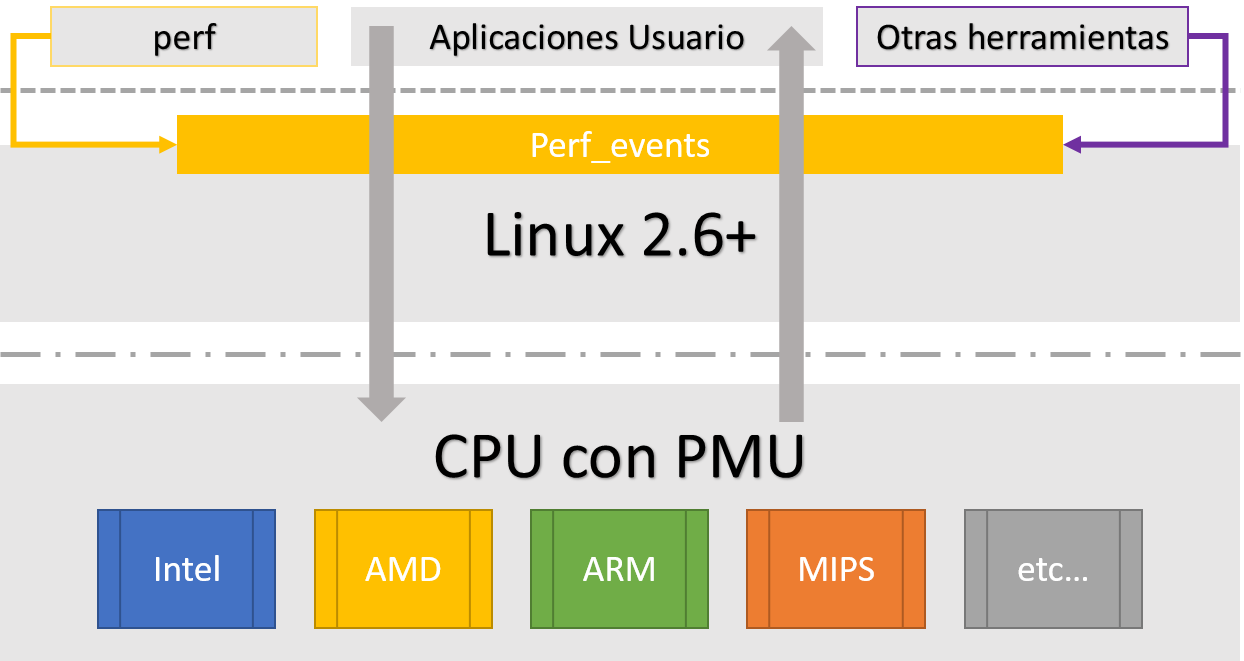
\includegraphics[scale=.45]{imagenes/perfArchitecture.png}
	\caption{Arquitectura de operación del framework provisto por \emph{Perf}.}
	\label{fig:perfFramework}
\end{figure}

Además de su gran capacidad para colectar datos, Perf es una herramienta de sencillo uso. Su funcionamiento se basa en la supervisión de un determinado proceso o tarea de la cual se construye un archivo con la información que se haya seleccionado a colectar \cite{article:perf}. Para ello, se pueden emplear las utilidades \verb=perf-record= y \verb=perf-stat= del framework las que trabajan supervisando un determinado proceso y proveyendo páginas de datos al espacio del kernel de Linux las cuales son escritas con información del sistema de dicho proceso, y son retornadas al espacio de usuario construyendo un informe a modo de output\footnote{La asignación del espacio de páginas a rellenar se hace por medio de la utilidad \verb=mmap= de Linux, que provee direcciones virtuales en un proceso para almacenar información.} (Ver figura \ref{fig:perfRecord}). Ésta característica es muy práctica pues sobre los reportes generados se pueden realizar operaciones de análisis más exhaustivos.

El potencial de ésta herramienta la perfila como una utilidad indispensable para el estudio en cuestión. En primer lugar por su capacidad de análisis de ejecución de código que permite obtener información cuantificada de las llamadas a sistema y de la dinámica del árbol de llamados\footnote{\emph{Call graph}, correspondiente a un grafo dirigido que representa la relación de llamados entre las subrutinas constitutivas de un proceso principal.} que permite reconocer la naturaleza de las funciones involucradas en el caso de estudio. En segunda instancia Perf es una estupenda herramienta para la recolección de datos de hardware al aprovechar el uso de la \emph{Performance Monitoring Unit (PMU)} del hardware del sistema, una característica que será revisada en detalle en secciones posteriores.

\begin{figure}[!h]
	\centering
	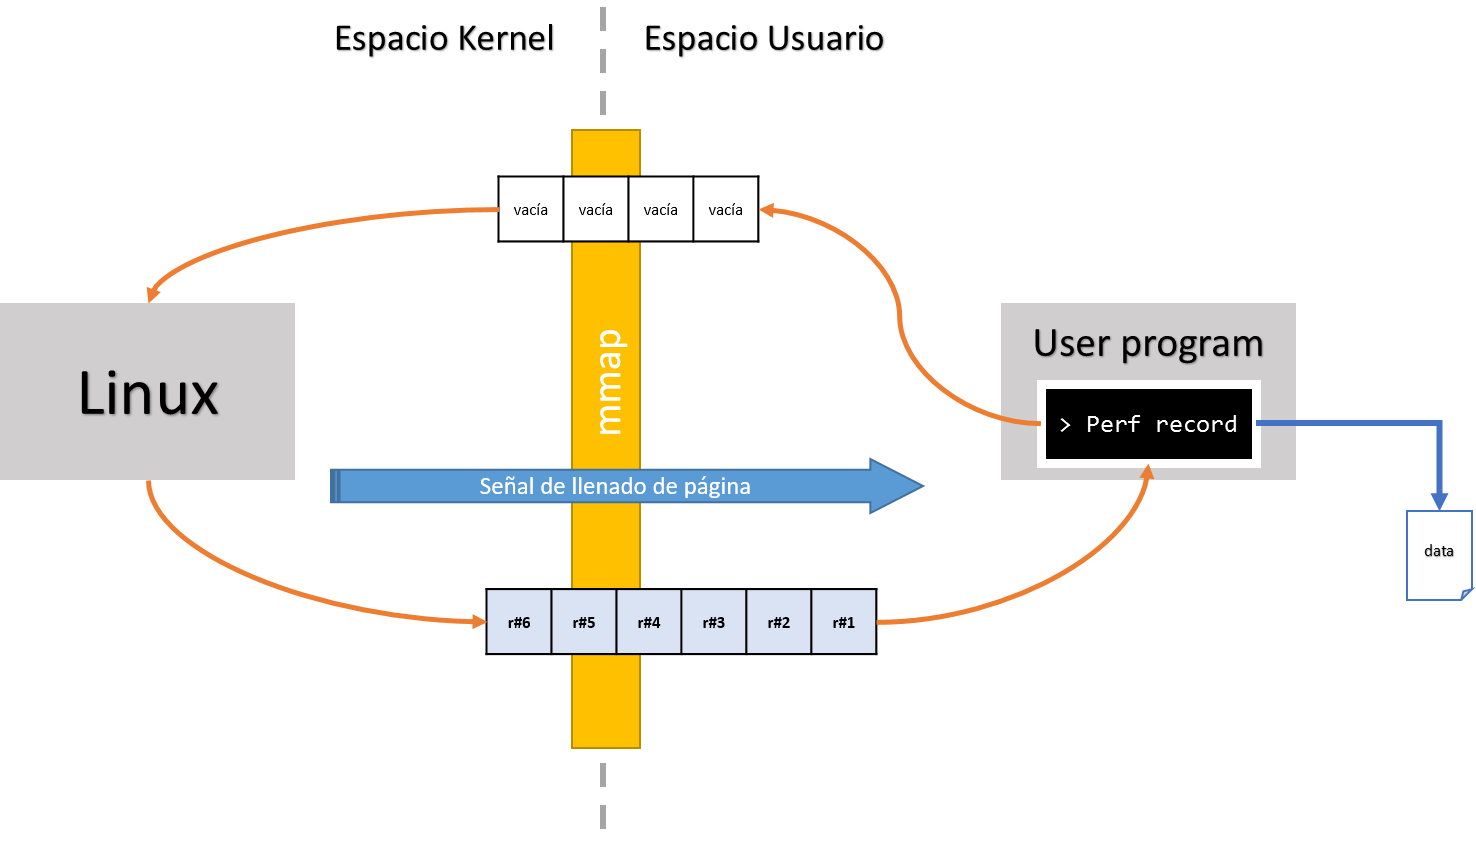
\includegraphics[scale=.52]{imagenes/perfRecord.png}
	\caption{Esquema de captura de datos de un programa usando el comando \emph{perf-record}.}
	\label{fig:perfRecord}
\end{figure}

\subsubsection{FTrace}
FTrace\footnote{\url{http://elinux.org/Ftrace}} es otra poderosa herramienta para análisis de rendimiento de software disponible para sistemas Linux \cite{paper:FTraceSony}. Su funcionamiento opera de naturaleza muy íntima con respecto al kernel mismo pues su recolección de datos se basa en el rastreo de la ejecución de funciones de forma dinámica en el espacio de kernel, caracterizando los tiempos reales de permanencia de cada llamada. Característica que lo hace una estupenda utilidad para el estudio de llamadas al sistema pudiendo recuperar datos como el tiempo de ejecución y cantidad de ocurrencia de las mismas.

Para su uso, FTrace opera como un verdadero framework del sistema sobre el kernel, del cual se pueden usar distintos métodos de rastreo de llamadas. Una de las funciones más poderosas de FTrace es el resultado que se puede obtener por medio de la instrumentación de código, que se refiere a la práctica de incorporar a los programas a analizar \emph{tracepoints} --o puntos de rastreo-- que son declaraciones explicitas de secciones de código a analizar y registrar. A pesar de que ésta característica es muy cómoda para programas propios, en el caso del análisis de funciones y llamadas de sistema propias del kernel de Linux, la instrumentación de código es una característica dispensable, siendo sólo necesaria la precisión de qué llamadas a sistema considerar en el análisis pues FTrace es flexible para hacer análisis directamente de funciones del sistema. El uso de ésta herramienta es muy flexible y configurable siendo activable a disposición del usuario, otra característica muy importante pues, al hacer una operación de rastreo de bajo nivel en el sistema, la actividad de FTrace significa una leve degradación en los tiempos netos de actividad de ciertas características del sistema.

El provecho que se puede sacar de ésta herramienta es usar su capacidad para cuantificar tiempo de funciones del kernel de Linux para estudiar la atomicidad de las llamadas bloqueantes del sistema. Así por ejemplo, se pretende determinar el tiempo que se pasa en estados bloqueantes de spinlocks (que terminan siendo pasos de \emph{busy-waiting}) en los cuales sólo se pierde tiempo por efectos de contención de recursos.

\section{Metodología de Experimentación}

Dado que la naturaleza de este estudio se relaciona con el comportamiento de funciones del sistema que administran las primitivas de acceso y sincronización, se realizarán las configuraciones pertinentes para cada herramienta a fin de contemplar dichos puntos de análisis. En el caso de Perf, la recolección de datos se realiza con la herramienta \verb=perf-record=, contemplando un post-procesamiento sobre los archivos de reporte generados a fin de colectar estadísticos asociados a las distintas funciones de manejo de spinlock antes mencionadas\footnote{Experimento \url{https://github.com/sebablasko/Test_MultiThreadStressTransmision} con privilegios de administrador.}.

Por otro lado, para el estudio con FTrace la configuración resulta un poco más compleja. Dado que es una herramienta de traceo dinámico que opera inspeccionando las llamadas de funciones de sistema, la activación de FTrace sobrecarga el funcionamiento del sistema general. Por ello, FTrace se debe activar y desactivar manualmente para analizar sólo los instantes de operación de la prueba de interés. Además, dado el amplio espectro de funciones disponibles para inspeccionar con el framework, se deben emplear las utilidades de filtrado de funciones a inspeccionar que provee el mismo framework, ello en pos de capturar funciones en línea con la dinámica del spinlock del Internet socket.

\vspace{1pc}
\begin{minipage}{\linewidth}
\begin{lstlisting}[style=BashInputStyle, label={code:ftrace}, caption={Configuración de filtros de FTrace sobre funciones a estudiar.}, captionpos=b]
[sebastian@labs-vhost ~]$ echo *spin* > /sys/kernel/debug/tracing/set_ftrace_filter 
[sebastian@labs-vhost ~]$ cat /sys/kernel/debug/tracing/set_ftrace_filter 
mutex_spin_on_owner
spin_msec
_spin_trylock
_spin_lock_irqsave
_spin_lock_irq
_spin_lock
_spin_unlock_irqrestore
_spin_lock_bh
_spin_trylock_bh
_spin_unlock_bh
bit_spin_lock
kvm_vcpu_on_spin
\end{lstlisting}
\end{minipage}

Por otra parte, el encendido y apagado del framework se configuró como parte del script de experimentación en el programa de la prueba\footnote{\url{https://github.com/sebablasko/Test_UDPTrace/}}. En el mismo, se configuró la opción \verb=set_ftrace_pid= para explicitar la inspección de FTrace sólo sobre el programa de la prueba, además del uso de la utilidad \verb=trace_marker= para instrumentar porciones de código de la prueba (como creación de threads, y término de consumo de datos) que permitiese una mayor facilidad al momento de estudiar los logs de ejecución recuperados.


\section{Resultados}
A continuación se ilustran los resultados experimentales obtenidos correspondientes a los datos colectados por Perf y FTrace. A modo de validación estadística, los resultados de las pruebas contemplan el promedio de un rango de 60 repeticiones en cada configuración dada por el caso de estudio.

\begin{figure}[!h]
	\centering
	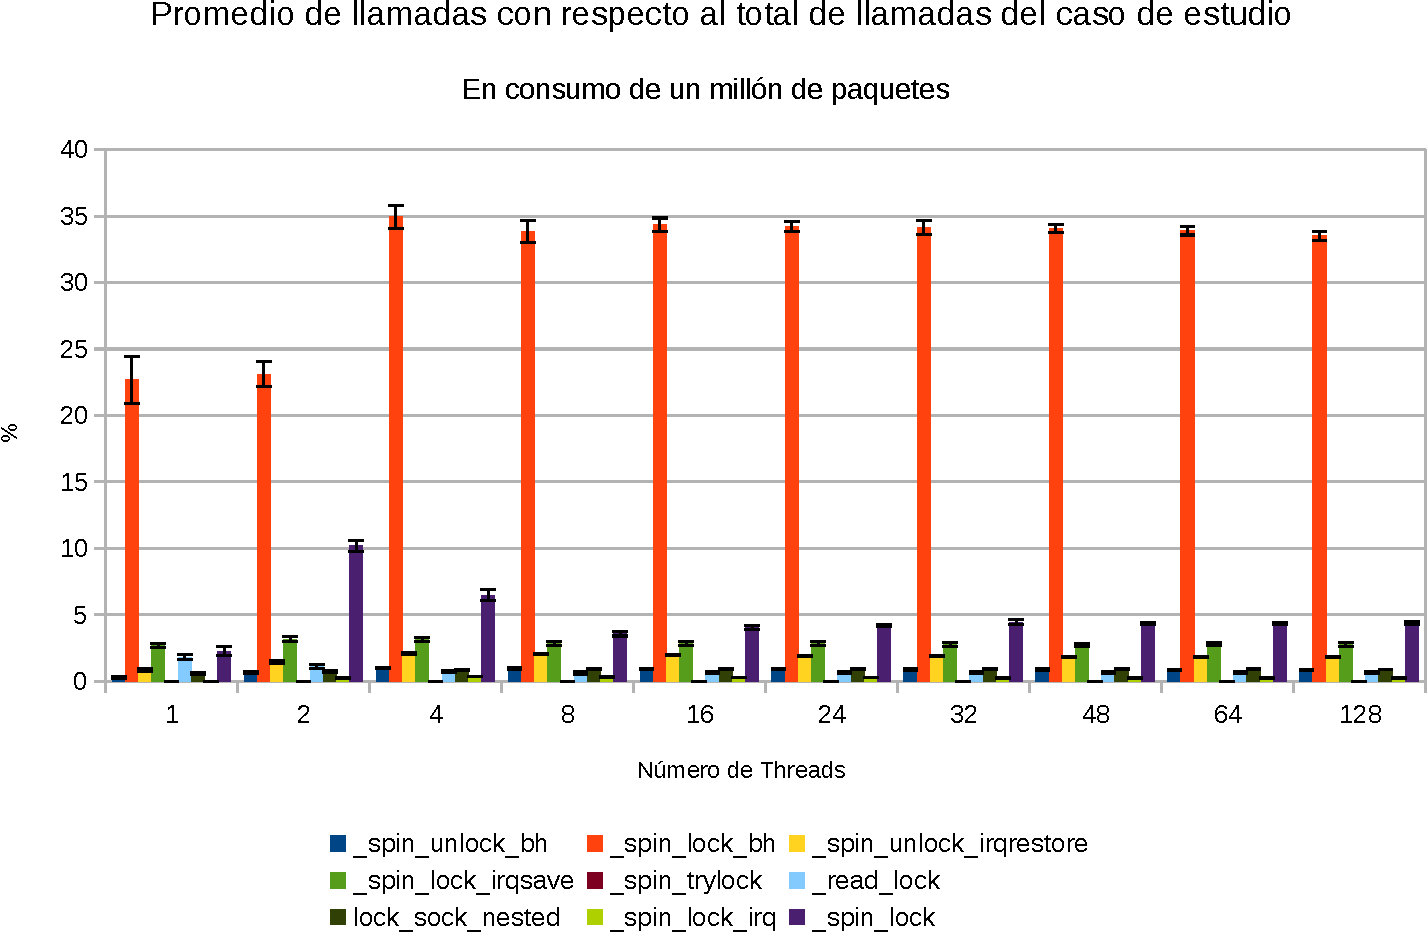
\includegraphics[scale=.6]{resultados/perfdetalle-crop.pdf}
	\caption{Resultados experimentales de los porcentajes de ejecución de las llamadas a sistema recolectadas por \emph{Perf}.}
	\label{fig:resPerf}
\end{figure}

\begin{figure}[!h]
	\centering
	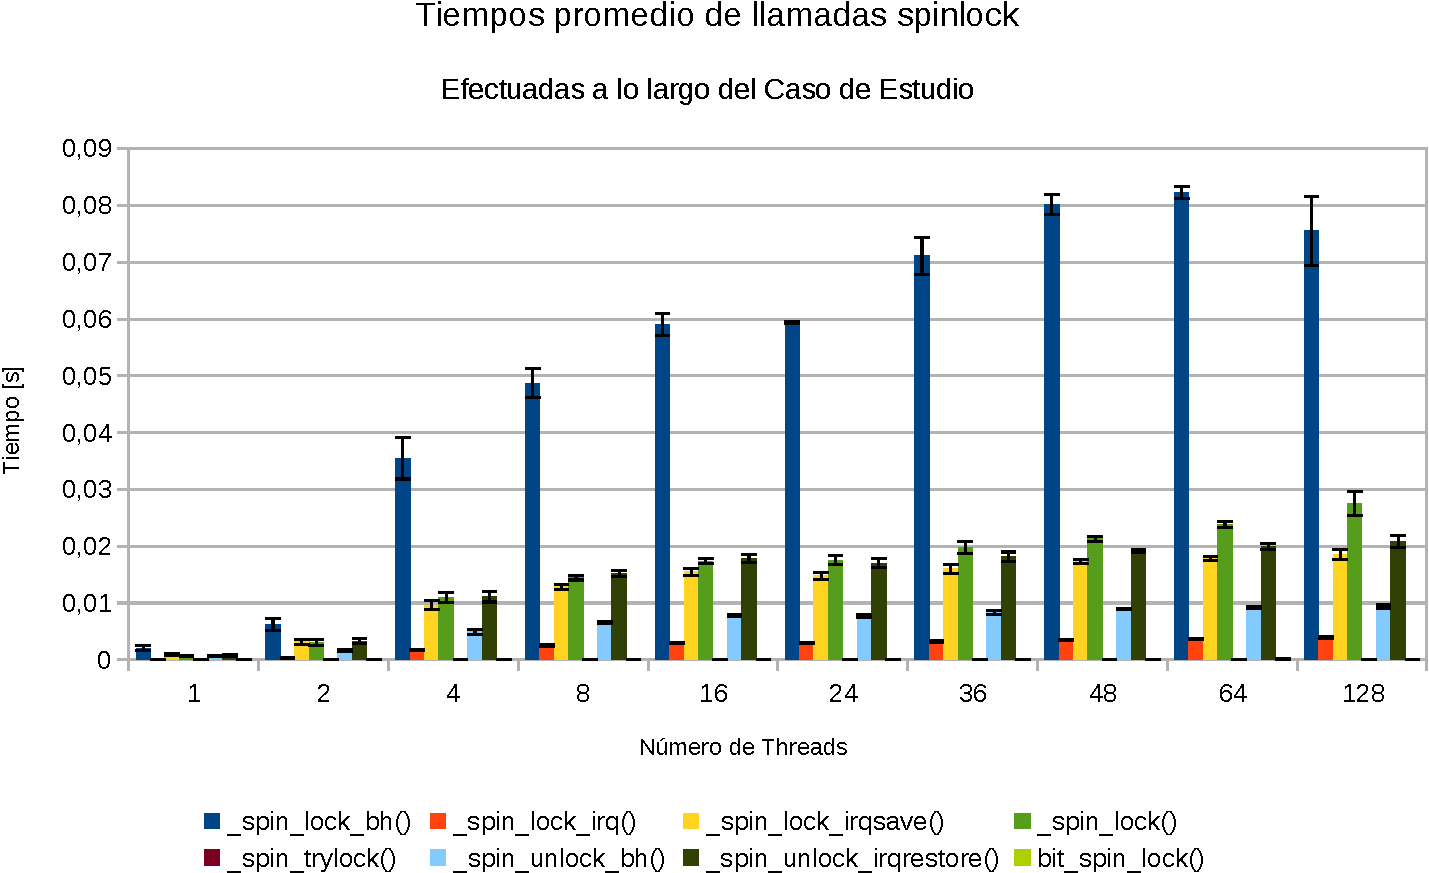
\includegraphics[scale=.6]{resultados/detalleFtrace-crop.pdf}
	\caption{Resultados experimentales de los tiempos de ejecución de las llamadas a sistema recolectadas por \emph{FTrace} para la adquisición y liberación del \emph{lock}.}
	\label{fig:detalleftrace}
\end{figure}


\section{Análisis y Discusión de Resultados}
A primera vista, los resultados corroboran una tendencia creciente de las operaciones (tanto en porcentaje como en tiempo neto de ejecución) de las operaciones de bloqueo sobre spinlock en las pruebas desarrolladas.

En el caso de los resultados de la prueba de Perf disponibles en la imagen \ref{fig:resPerf}, se puede apreciar un comportamiento dominante en el porcentaje de llamado de funciones de una de las funciones por sobre las demás: \textbf{\_spin\_lock\_bh}, llamada que en condiciones de concurrencia puede aumentar su porcentaje de presencia en la ejecución desde un 22\% a casi un 35\%. Otro punto interesante es que, a medida a medida que el escenario se vuelve más competitivo para los threads, los porcentajes rescatados por ésta prueba para llamadas de bloqueo aumentan hasta aproximadamente los 4 threads, desde donde se estabiliza, manteniéndose sobre el 40\% sólo en éste apartado.

\begin{figure}[!h]
	\centering
	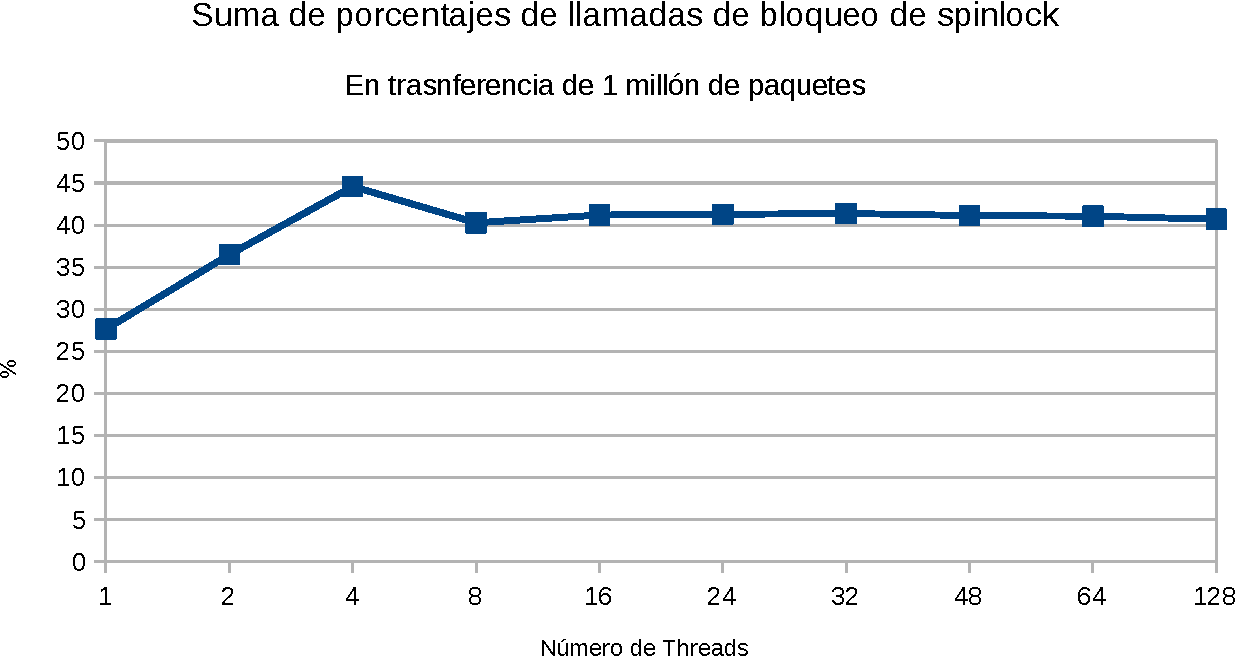
\includegraphics[scale=.6]{resultados/sumaperf-crop.pdf}
	\caption{Gráfico de suma de porcentajes de llamadas de bloqueo del \emph{lock} de spinlock.}
	\label{fig:sumaperf}
\end{figure}

Para reconocer mejor la dinámica de consumo de tiempos en las funciones inspeccionadas en el caso de estudio, se usaron los reportes generados por Perf para construir un nuevo tipo de visualización de llamadas a sistema: Un \emph{Call-Graph-Chart} (Ver imagen \ref{fig:callgraph}), de manera de poder reconocer los bloques de funciones más repetidos en la ejecución del caso de prueba. Para ésta visualización se aprovechó el script \emph{gprof2dot}\footnote{\url{https://github.com/jrfonseca/gprof2dot}}. En éste caso, resulta evidente cómo el grafo de llamadas de sistema se complejiza drásticamente al incorporar más threads, de la mano con el aumento en los porcentajes de permanencia en llamadas de sincronización.

\begin{figure}[!h]
	\centering
	
\includegraphics[scale=.5]{imagenes/fcfm}
	\caption{Visualización de call-graph identificando las llamadas a sistema y sus pesos en el caso de prueba.}
	\label{fig:callgraph}
\end{figure}

Lo anterior postula una primera relación entre el número de threads en el acceso concurrente al socket con respecto al porcentaje y dinámica de llamados a funciones de bloqueo del spinlock. Sin embargo, los porcentajes de llamadas no son del todo relevantes si no se saben los tiempos efectivos que significan en la prueba. Para ello, se repasan los resultados de Ftrace.

Los resultados generales obtenidos con el estudio de FTrace disponibles en la figura \ref{fig:detalleftrace} dan cuenta de un fenómeno aún más interesante. Al igual que con los datos colectados con Perf, se ilustra una estrecha relación entre los tiempos de operación de las funciones relacionadas a spinlock a medida que se van incorporando threads, sin embargo, en éste caso, la tendencia resulta siempre creciente, plasmando cómo a medida que se van usando más threads, el sistema operativo pasa más tiempo en tareas de coordinación en su acceso.

Por otro lado, al realizar una colección de datos con FTrace a modo de recuperar el total de tiempo que se pasa en operaciones de tipo de bloqueo de spinlock se obtiene el resultado ilustrado en la imagen \ref{fig:sumaFtrace}. Una característica interesante de éste resultado es que, la tendencia de tiempos producida tiene un ajuste de naturaleza logarítmica, con un índice de determinación superior al 96\%. Éste resultado es muy significativo, pues revela que los tiempos reales de acción de las funciones de bloqueo de spinlock siguen una tendencia de la misma naturaleza a los tiempos netos de operación del caso de estudio, estipulando una relación estrecha entre ambos y postulando como principal responsable de los tiempos finales a las funciones de coordinación en el acceso al spinlock.

\begin{figure}[!h]
	\centering
	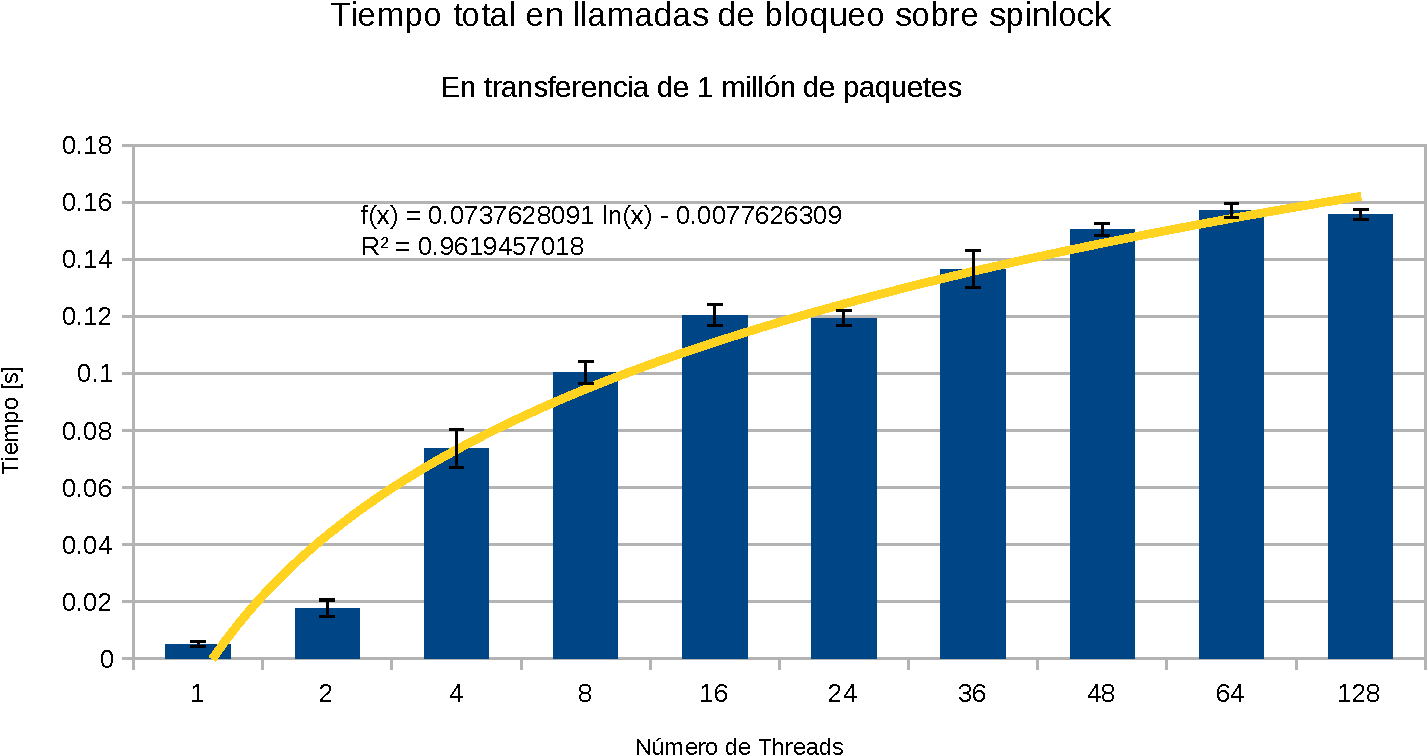
\includegraphics[scale=.5]{resultados/sumaFtrace-crop.pdf}
	\caption{Tiempos totales de bloqueo sobre el \emph{lock} por las distintas llamadas de sistema capturadas por \emph{Ftrace} en el caso de estudio juntos con una curva de aproximación de tendencia.}
	\label{fig:sumaFtrace}
\end{figure}
Más aún, si se repasan las tendencias de cada una de las principales llamadas de bloqueo y de liberación de spinlock (ver figura \ref{fig:Ftracebloquealibera}) se puede ver como las tendencias de naturaleza logarítmica prevalecen al aumentar el número de threads en el consumo de datos. Sin perjuicio de lo anterior, otro dato interesante es que las operaciones de liberación (Fig. \ref{fig:ftracelibera}) son muchísimo más cortas que las de bloqueo (Fig. \ref{fig:ftracebloquea}) revelando el escenario de competencia al que se ve enfrentado el spinlock ante la concurrencia en el acceso.

\begin{figure}[h!]
	\centering
	\hspace*{\fill}
	\subfigure[Funciones de Bloqueo]{
		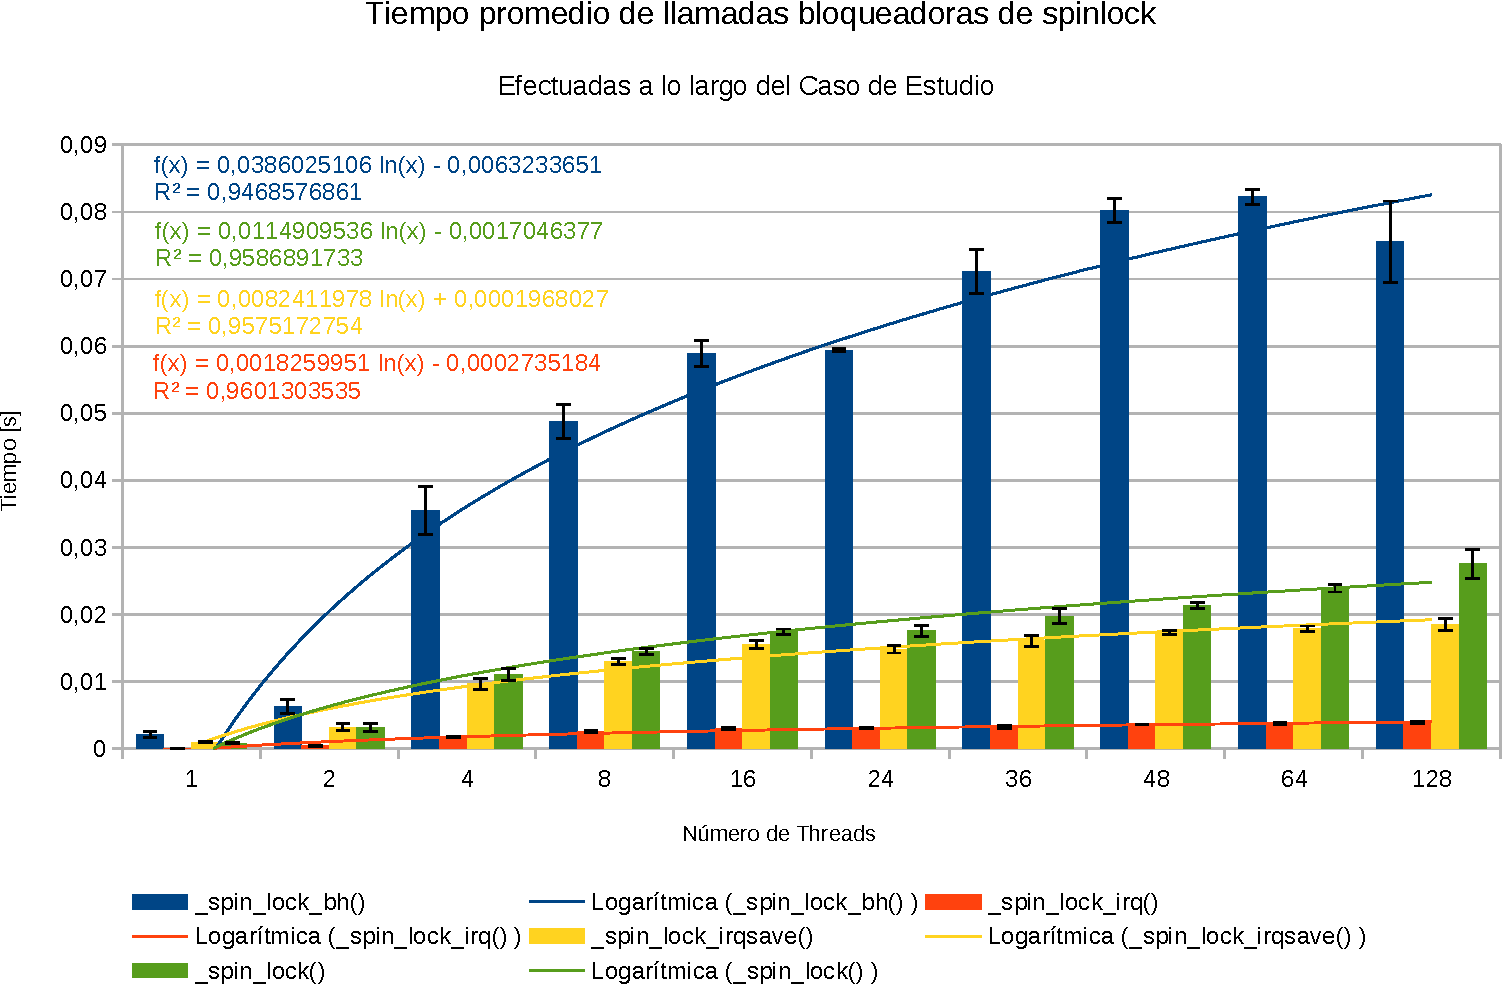
\includegraphics[width=.47\textwidth]{resultados/bloqueantesftrace-crop.pdf}
		\label{fig:ftracebloquea}
	}\hfill
	\subfigure[Funciones de Liberación]{
		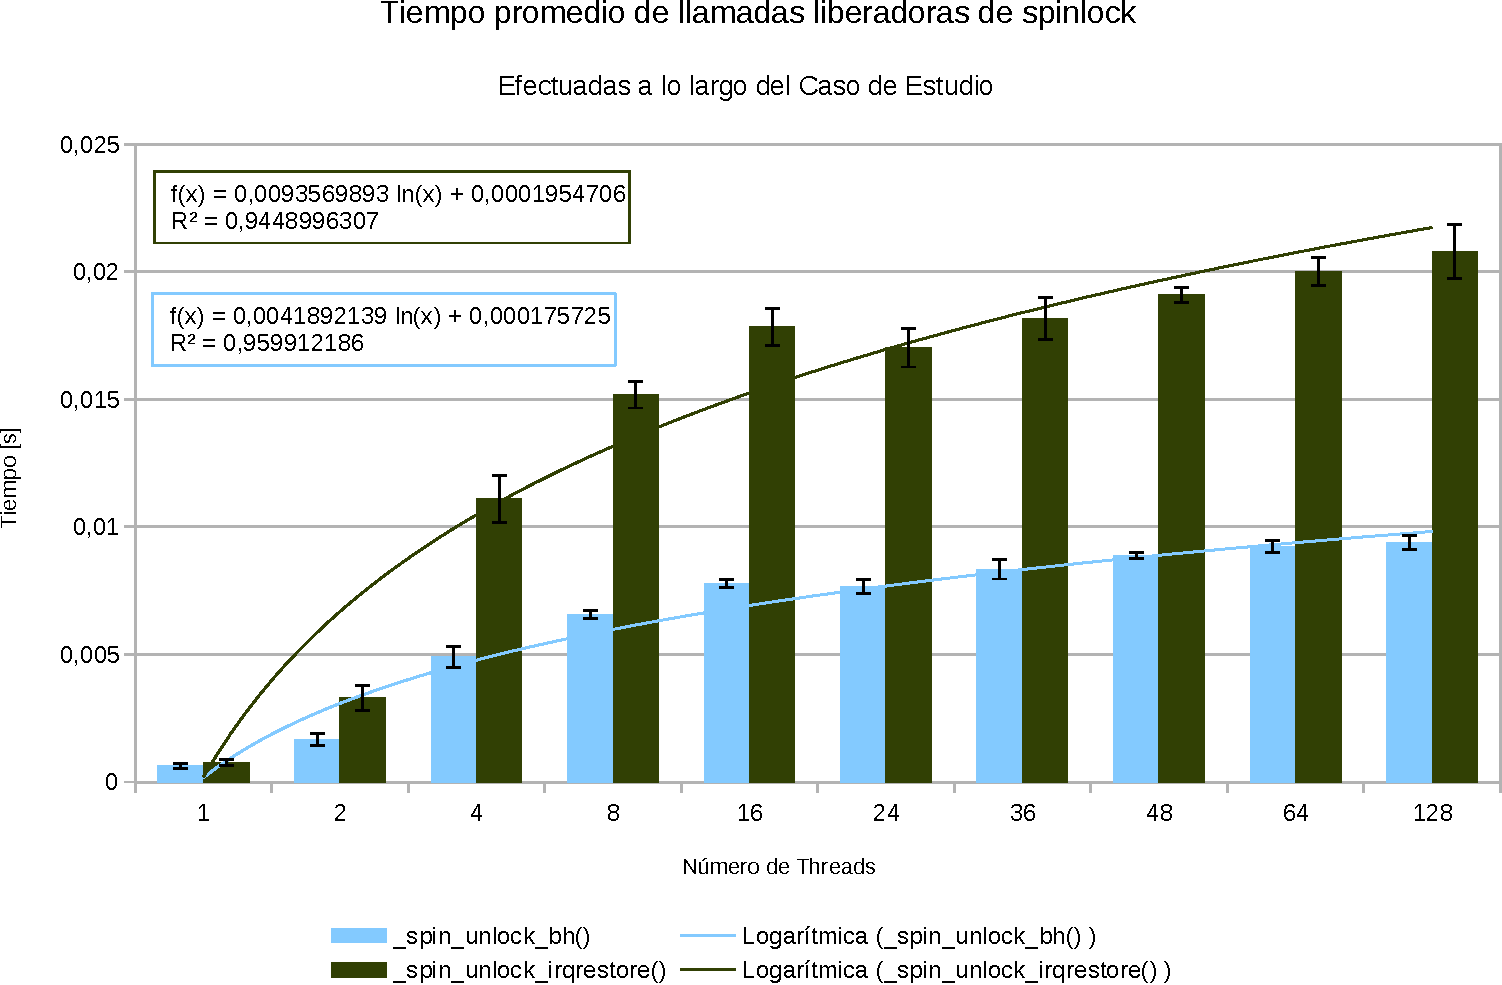
\includegraphics[width=.47\textwidth]{resultados/liberadorasFtrace-crop.pdf}
		\label{fig:ftracelibera}
	}
	\caption{Graficos con tendencias de tiempos del lock capturados con \emph{Ftrace} a lo largo del caso de estudio.}
	\label{fig:Ftracebloquealibera}
	\hspace*{\fill}
\end{figure}

\subsection{TraceDisplay}
Para poder obtener una interpretación adicional del fenómeno reconocido, se construyó una herramienta de visualización de las llamadas a sistema para funciones de sincronización que permitiese reconocer las porciones de tiempo que tomasen en cada procesador dichas funciones. Para ello, la herramienta denominada \emph{TraceDisplay} recibe un log generado con \emph{FTrace} que incluya las llamadas de sistema ya filtradas, y construye un mapa de tiempo coloreado donde se pueden apreciar las porciones de tiempo que consume cada llamada y desde cual CPU se originan. El resultado se puede apreciar en la imagen \ref{fig:traceDisplay} donde se ilustra el caso de analizar los logs generados por FTrace en un escenario de acceso de 4 threads en el caso de estudio.

Éste subproducto de la investigación principal junto con su documentación de uso está publicado\footnote{Disponible en \url{https://github.com/sebablasko/TraceDisplay}} y disponible para su uso.

\begin{figure}[!h]
	\centering
	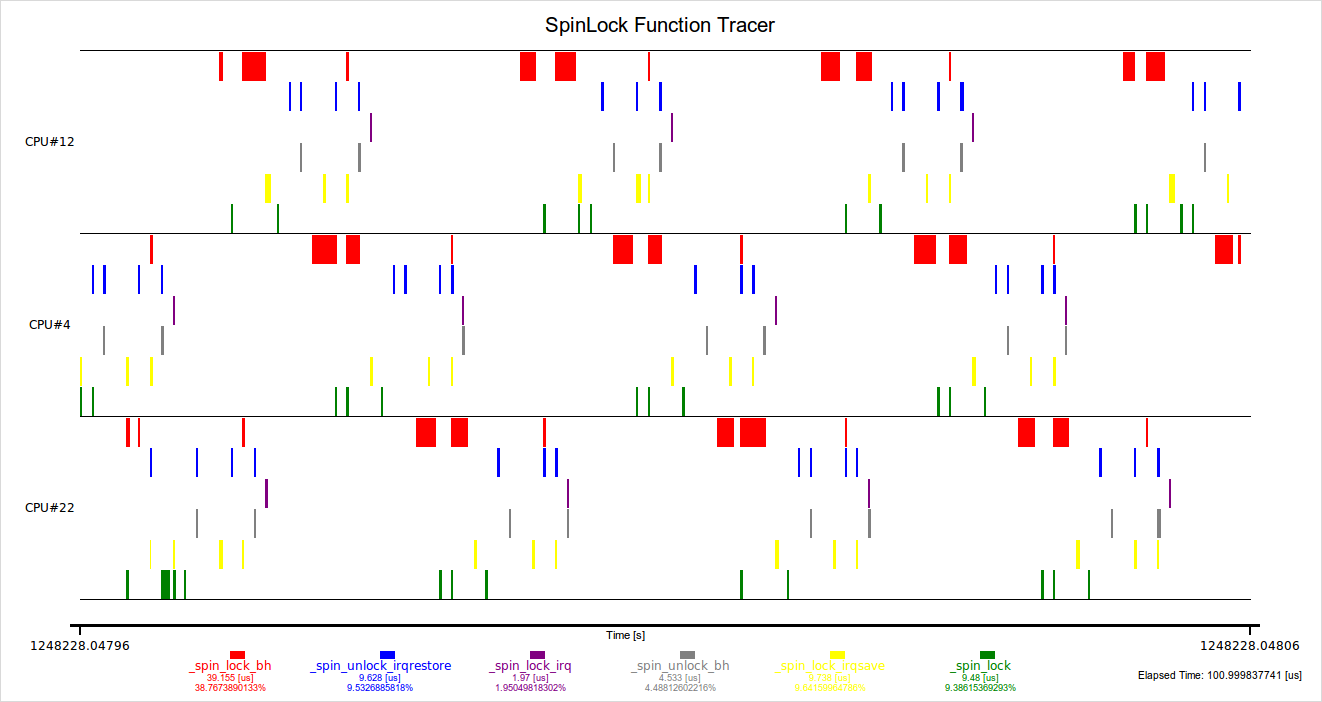
\includegraphics[scale=0.34]{imagenes/traceVisualization.png}
	\caption{Visualización de aplicación de llamadas de sistema de sincronización realizadas entre procesadores, generada con la herramienta TraceDisplay.}
	\label{fig:traceDisplay}
\end{figure}

Resultados como el mostrado en la figura \ref{fig:traceDisplay} ilustran como en la práctica, las operaciones de bloqueo se terminan ejecutando secuencialmente, aun cuando son distintos los CPU que los originen. Esto producto de que es una misma estructura la que se está compartiendo la cual no tiene un soporte adecuado para permitir modificaciones concurrentes de orígenes distintos, generando así un sobrecosto producido por dicha serialización en el acceso.


\section{Conclusiones}
A raíz del estudio de operación de primitivas de sincronización del sistema se pueden rescatar varios aspectos interesantes:
\begin{itemize}
\item La tendencia en los costos de tiempo son crecientes a medida que se agregan hilos que consumen el mismo socket. Ello tanto en porcentaje de llamadas de sistema, como también en tiempos netos en dichas llamadas.
\item Se destacan estructuras de tipo spinlock como las más reiteradas en el rastro de llamadas a sistema para la aplicación de mecanísmos de protección en el caso de estudio. En particular, la llamada a sistema \textbf{\_spin\_lock\_bh} es la más significativa en la operación de los mecanismos de acceso y toma del \emph{lock} que protege al Internet socket.
\item Se reconoce una significativa diferencia entre los tiempos y porcentajes de llamadas a sistema de tipo bloqueante por sobre los de tipo liberador del \emph{lock}, escenario que da cuenta de la situación de competencia que empeora a medida que se incluyen más threads en la prueba.
\item Se destaca una tendencia de naturaleza logarítmica en el crecimiento de tiempos que toman las llamadas bloqueantes sobre el spinlock del socket, ajustada con un coeficiente de determinación superior al 96\% y que sigue la misma tendencia de los tiempos netos reconocidos en el caso de estudio.
\end{itemize}
A raíz de lo anterior, se reconoce en el spinlock de protección del socket como un punto de cuello de botella al momento de emplear accesos concurrentes a una estructura socket. Ello al actuar como un punto de bloqueo que termina serializando el acceso al consumo de datos y que, lejos de reducir los tiempos paralelizando el acceso, los aumenta, producto de la serialización y de la responsabilidad de coordinar los hilos, propios de éste escenario.